\documentclass[11pt, a4paper]{article}
\usepackage{pythontex}
\usepackage[german]{babel}
\usepackage{graphicx}
\usepackage{tabularx}
\usepackage{hyperref}
\usepackage{lastpage}
\usepackage[parfill]{parskip}
\usepackage{fancyhdr}
\usepackage{pythontext}
\usepackage[headheight=55pt,
 left=25mm, bottom =25mm]{geometry}

%%%%%% SANS SERIF FONT %%%%%%%%
%\usepackage[OT1]{fontenc}
%\renewcommand*\familydefault{\sfdefault}

%Header Customization
\fancyhead[L]{
\includegraphics[width=0.23\linewidth]{phytax_logo.jpg} \\
}
\fancyhead[C]{\footnotesize
\begin{tabular}{ l }
 Phytax GmbH \\ 
 Wagistrasse 23 \\  
 CH-8952 Schlieren 
\end{tabular}
}

\fancyhead[C]{\footnotesize
 Phytax GmbH \\ 
 Wagistrasse 23 \\  
 CH-8952 Schlieren 
}
\fancyhead[R]{ \footnotesize \noindent \href{mailto:info@phytax.ch}{info@phytax.ch} \\
\href{http://www.phytax.ch}{www.phytax.ch}\\
\href{tel:41434950430}{+41 (0) 43 495 04 30}}

\pagestyle{fancy}
\lfoot[]{\footnotesize Validierungsplan PHYDENT-\DatumRelease}
\rfoot[]{\thepage/\pageref{LastPage} }
\cfoot{}
\renewcommand{\headrulewidth}{0pt}
%%%%%%%%%%%%%%%% VARIABLEN %%%%%%%%%%%%%%%%%%%%%%%%%%%%%
\newcommand\VersionPhEur{10.5}
\newcommand\DatumRelease{20210929}
\newcommand\AnzahlProdukte{227}

\newcommand\NoSpectraRefLearn{5200 (54.2\%)}
\newcommand\NoSpectraRefVal{200 (20.8\%)}
\newcommand\NoSpectraPruef{2400 (25.0\%)}
\newcommand\NrSpektren{7128}
\newcommand\Granulatchargen{396}
\newcommand\NrMatrix{72}
\newcommand\DateRange{2020-2021}


\begin{document}
\section*{Validierungsplan für Prüfungsmethode: PHYDENT-\DatumRelease }

\renewcommand{\arraystretch}{1.2}
\begin{center}
\begin{tabular}{| m{3.5cm} | m{3.5cm}| m{3.5cm} |m{3.5cm}|}
\hline
 & Person & Datum & Visum \\
\hline
Erstellt & & &  \\
& & &\\
\hline
Geprüft & & & \\
& & & \\
\hline
Freigegeben & & & \\
&&&\\
\hline
\end{tabular}
\end{center}









\subsection*{Zusammenfassung}
PHYDENT ist eine chemometrische Prüfmethode für die Identifikation von Granulaten der Traditionellen Chinesischen Medizin (TCM). PHYDENT ist vorgesehen für die Ausgangstoffprüfung gemäß deutscher Apothekenbetriebsordnung (§§ 6, 7 und 11). Die Prüfmethode ist ausgelegt für die Identifikation von Granulatprodukten verschiedener Hersteller basierend auf spektralen Merkmalen im Mittleren Infrarot (MIR; 400–4000 cm$^{-1}$). Die Methode wurde entwickelt zur Verwendung mit Infrarot-Spektrometern der ALPHA Produktereihe (Bruker, Deutschland). Dieses Dokument beschreibt den Validierungsplan für PHYDENT gemäß ICH (Q2)R1 sowie den Bestimmungen des Europäischen Arzneibuchs (\VersionPhEur). Die Methodenvalidierung umfasst Prüfungen zu Spezifität und weiteren kritischen Parametern.


\subsection*{Zweck}
Dieser Validierungsplan beschreibt die analytische Testmethode PHYDENT-20210929, im Folgenden PHYDENT genannt, sowie die Strategie und Akzeptanzkriterien für deren Validierung.

\newpage
\tableofcontents

\newpage

\section{Beschreibung der Methode}
PHYDENT ist eine computergestützte chemometrische Methode für die infrarotspektroskopische Identifikation von Granulaten der Traditionellen Chinesischen Medizin\footnote{Bei Granulaten handelt es sich in der Regel um wässrige Rohdrogen-Extrakte, welche auf eine Trägersubstanz (z.B. Maisstärke) aufgezogen sind.}. Die Methode ist ausgelegt für die Identifikation von 227 Granulatprodukten unterschiedlicher Hersteller nach deutscher Apothekenbetriebsordnung\footnote{TCM-Granulate gelten als Ausgangstoffe im Sinne der ApBetrO § 7, da Patienten üblicherweise Rezepturen aus mehreren Granulaten verschrieben werden. Demzufolge ist auch bei Vorliegen eines GMP-konformen Prüfzertifikats für jedes Rezepturgranulat eine nochmalige Identitätsprüfung in der Apotheke erforderlich (ApBetrO §§ 6 \& 11).}.  PHYDENT stellt gemäß Ph.Eur. (\VersionPhEur; 5.21) eine Analyse mit Kontrollfunktion dar, bei welcher die Zugehörigkeit zu bekannten Klassen vorhergesagt wird. Die Eingabedaten der Prüfmethode sind spektrale Probenmerkmale im Mittleren Infrarot (MIR, 400 - 4000 cm$^-{1}$), die Ausgabe ist die Produkteidentität von TCM Granulaten.


\subsection{Geltungsbereich}

\textbf{Proben}: PHYDENT ist ausgelegt für die Identifikation von definierten Chargen von 227 Granulatprodukten unterschiedlicher Hersteller (Anhang 3, 4)\footnote{Die Identifikation von unbekannten Chargen ist nicht vorgesehen. Grund hierfür ist, trotz standardisierter Herstellungsbedingungen dass mehrere Chargen desselben Produkts signifikante spektrale Variabilität aufweisen können (z.B. aufgrund von Unterschieden in den dafür verwendeten Rohstoffen).}.  Die Methode muss fähig sein, unbekannte Gebinde dieser Chargen zu identifizieren (Generalisierung auf Ebene des Gebindes). \\

\textbf{Gerät/Analyst}: Die Methode ist vorgesehen für die Verwendung mit der ALPHA/Platinum-ATR-Messplattform (Bruker). Die Methode muss Unabhängig des Geräts und unabhängig des Analysten dieselben Resultate erzielen (Generalisierung auf Ebene des Geräts und des Analysten).

\textbf{Verwendungsszenario} (Abbildung (\ref{fig:Flussdiagram})):
\begin{enumerate}
\item Ein TCM-Granulat wird an eine Apotheke geliefert. Der Lieferung liegt ein GMP-konformes Prüfzertifikat bei. Das Zertifikat bezeugt unter anderem die Arzneibuch-konforme Identifikationprüfung der Charge mittels Hochleistungsdünnschichtchromatographie (2.8.25).
\item Die Wareneingangskontrolle und Probennahme der zu prüfenden Granulate erfolgt nach apothekeninternem Qualitätssicherungssystem.
\item Das versiegelte Gebinde wird geöffnet und eine kleine Probenmenge (Spatelspitze) zur Messung entnommen. Die Messung wird auf der ALPHA/Platinum ATR Messplattform ausgeführt (Bruker, Deutschland).
\item Direkt im Anschluss an die Messung identifiziert die jeweils aktuelle Version von PHYDENT automatisch das Granulatprodukt. Die Analyseergebnisse werden gespeichert und werden dokumentiert.
\end{enumerate}

\begin{figure}
\centering
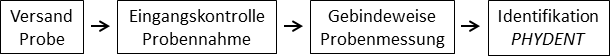
\includegraphics[width=0.8\textwidth]{flussdiagram.png}
\caption{Flussdiagramm Verwendungsszenarion}
\label{fig:Flussdiagram}
\end{figure}

\subsection{Referenzen}
TCM-Granulate gelten gemäß Europäischem Arzneibuch als „Extrakte aus pflanzlichen Drogen“ (\VersionPhEur; 0765). Für Granulate liegen keine Einzelmonographien vor. Deshalb können für Infrarot-basierte Identifikationsmethoden gemäß Europäischem Arzneibuch (\VersionPhEur; 2.2.24) geeignete Referenzstandards definiert und verwendet werden.

\subsubsection{Granulate}
Alle Produktchargen wurden durch Phytax GmbH gemäß den Bestimmungen des jeweils aktuellen Europäischen Arzneibuchs (0765; 2.8.25), sowie nach internen Qualitätsmanagementsystem (SOPs 3.2.3, 3.6.6 und 3.6.7) einwandfrei geprüft. Die Prüfung der Referenzen erfolgte jeweils zusammen mit dem entsprechenden, durch den Granulathersteller zur Verfügung gestellten, Ausgangsmaterial (Rohdroge). Somit ist die Rückverfolgbarkeit auf das jeweilige Ausgangsmaterial gewährleistet.

\subsubsection{Hilfsstoffe}
\label{sec:Hilfsstoffe}
Die für die Granulat-Produktepalette verwendeten Hilfsstoffe sind Cellulose, Cyclodextrin, Laktose und Maisstärke. Diese Hilfsstoffe werden in der Methodenentwicklung und Methodenprüfung berücksichtigt (vgl. Kap. 1.3.1).

\subsection{Spektraldaten}
Die Probenmessung erfolgte gemäß internem Qualitätsmanagementsystem (SOP 3.7.1) sowie den Bestimmungen des jeweils gültigen Europäischen Arzneibuchs (2.2.24). Für die Modellierung von PHYDENT wurden insgesamt \NrSpektren\ Spektren von \Granulatchargen\ Granulatchargen (\AnzahlProdukte\ Produkte) verwendet (Anhänge 3, 4). Nebst diesen Produktspektren wurden insgesamt \NrMatrix\ Spektren von vier in der Granulatherstellung gängig verwendeten Hilfsstoffen einbezogen. Die Spektraldaten wurden ausgewogen auf zwei baugleichen Spektrometern (ALPHA / Platinum ATR; Bruker) durch fünf Analysten \DateRange\ gemessen (Anhang 8).

\subsubsection{Sampling Design}
Der Datensatz zur Entwicklung der Methode (Lern-/Validierungsdaten) besteht aus insgesamt 7200 Spektren (Anhang 5), wobei die Lerndaten und Validierungsdaten in einem Verhältnis von 73.2:27.8. aufgeteilt wurden. Zur Überprüfung der Leistungsfähigkeit der Methode sollen ferner unabhängige Prüfdaten mit einem Umfang von mindestens 20\% der L/V-Daten verwendet werden (Tabelle \ref{tab:Aufteilung_gesamtdaten}). Der gesamte Datensatz soll ausgeglichen auf zwei baugleichen Spektrometern gemessen werden (Generalisierung auf Geräteebene). Abbildung \ref{fig:Sampling_Design} zeigt eine Übersicht des angewendeten Sampling Designs.

\begin{table}
\begin{center}
\begin{tabular}{| m{7cm} | m{7cm}| }
\hline
Datensatz & Anzahl Spektren \\
\hline
1) Lerndaten & \NoSpectraRefLearn \\
\hline
2) Validierungsdaten (hold-out) & \NoSpectraRefVal \\
\hline
3) Unabhängige Prüfdaten & \NoSpectraPruef \\
\hline
\end{tabular}
\end{center}
\caption{Aufteilung der Gesamtdaten zur Entwicklung und Überprüfung der Methode}
\label{tab:Aufteilung_gesamtdaten}
\end{table}

\textbf{Produkte}\\[1.2pt]
Gemäß Anwendungsszenario muss PHYDENT fähig sein, unbekannte Gebinde von bekannten bzw. unterstützen Produktechargen zu erkennen (Generalisierung auf Gebindeebene). Deshalb werden den Lern- \& Validierungsdaten (L\&V) und den Prüfdaten (P) für jede Produktecharge unabhängige Gebinde zugewiesen. Für die L\&V-Daten wurde pro Produktecharge ein Gebinde gemessen; für die P-Daten werden zusätzliche ein weiteres unabhängige Gebinde gemessen (pro Gerät je 3-fach wiederholt).

\textbf{Hilfsstoffe}\\[1.2pt]
Granulat-Hilfsstoffe sind potentielle Verfälschungen von Granulatprodukten und werden deshalb in der Methodenentwicklung einbezogen (Negativkontrolle). Total \NrMatrix\ Spektren der in Kap. \ref{sec:Hilfsstoffe} beschriebenen Hilfsstoffe wurden ausgewogen auf zwei baugleichen Spektrometern gemessen (pro Charge je 6-fach wiederholt) und den L\&V- Daten zugewiesen. Unabhängige Messungen derselben Hilfstoffe werden den P-Daten zwecks besserer Identifikation bzw. Zurückweisung zugewiesen.

\textbf{Blank}\\[1.2pt]
Messung des unbedeckten Sensors (Leermessung/Blank) ist ein möglicher Messfehler. Um falsche Identifikationsresultate aufgrund einer unbeabsichtigten Leermessung auszuschliessen, werden Blank-Messungen den P-Daten zugewiesen (Negativkontrolle). Blankmessungen wurden auf zwei baugleichen Spektrometern erstellt (je 6-fach wiederholt).
 
\begin{figure}[h]
\begin{center}
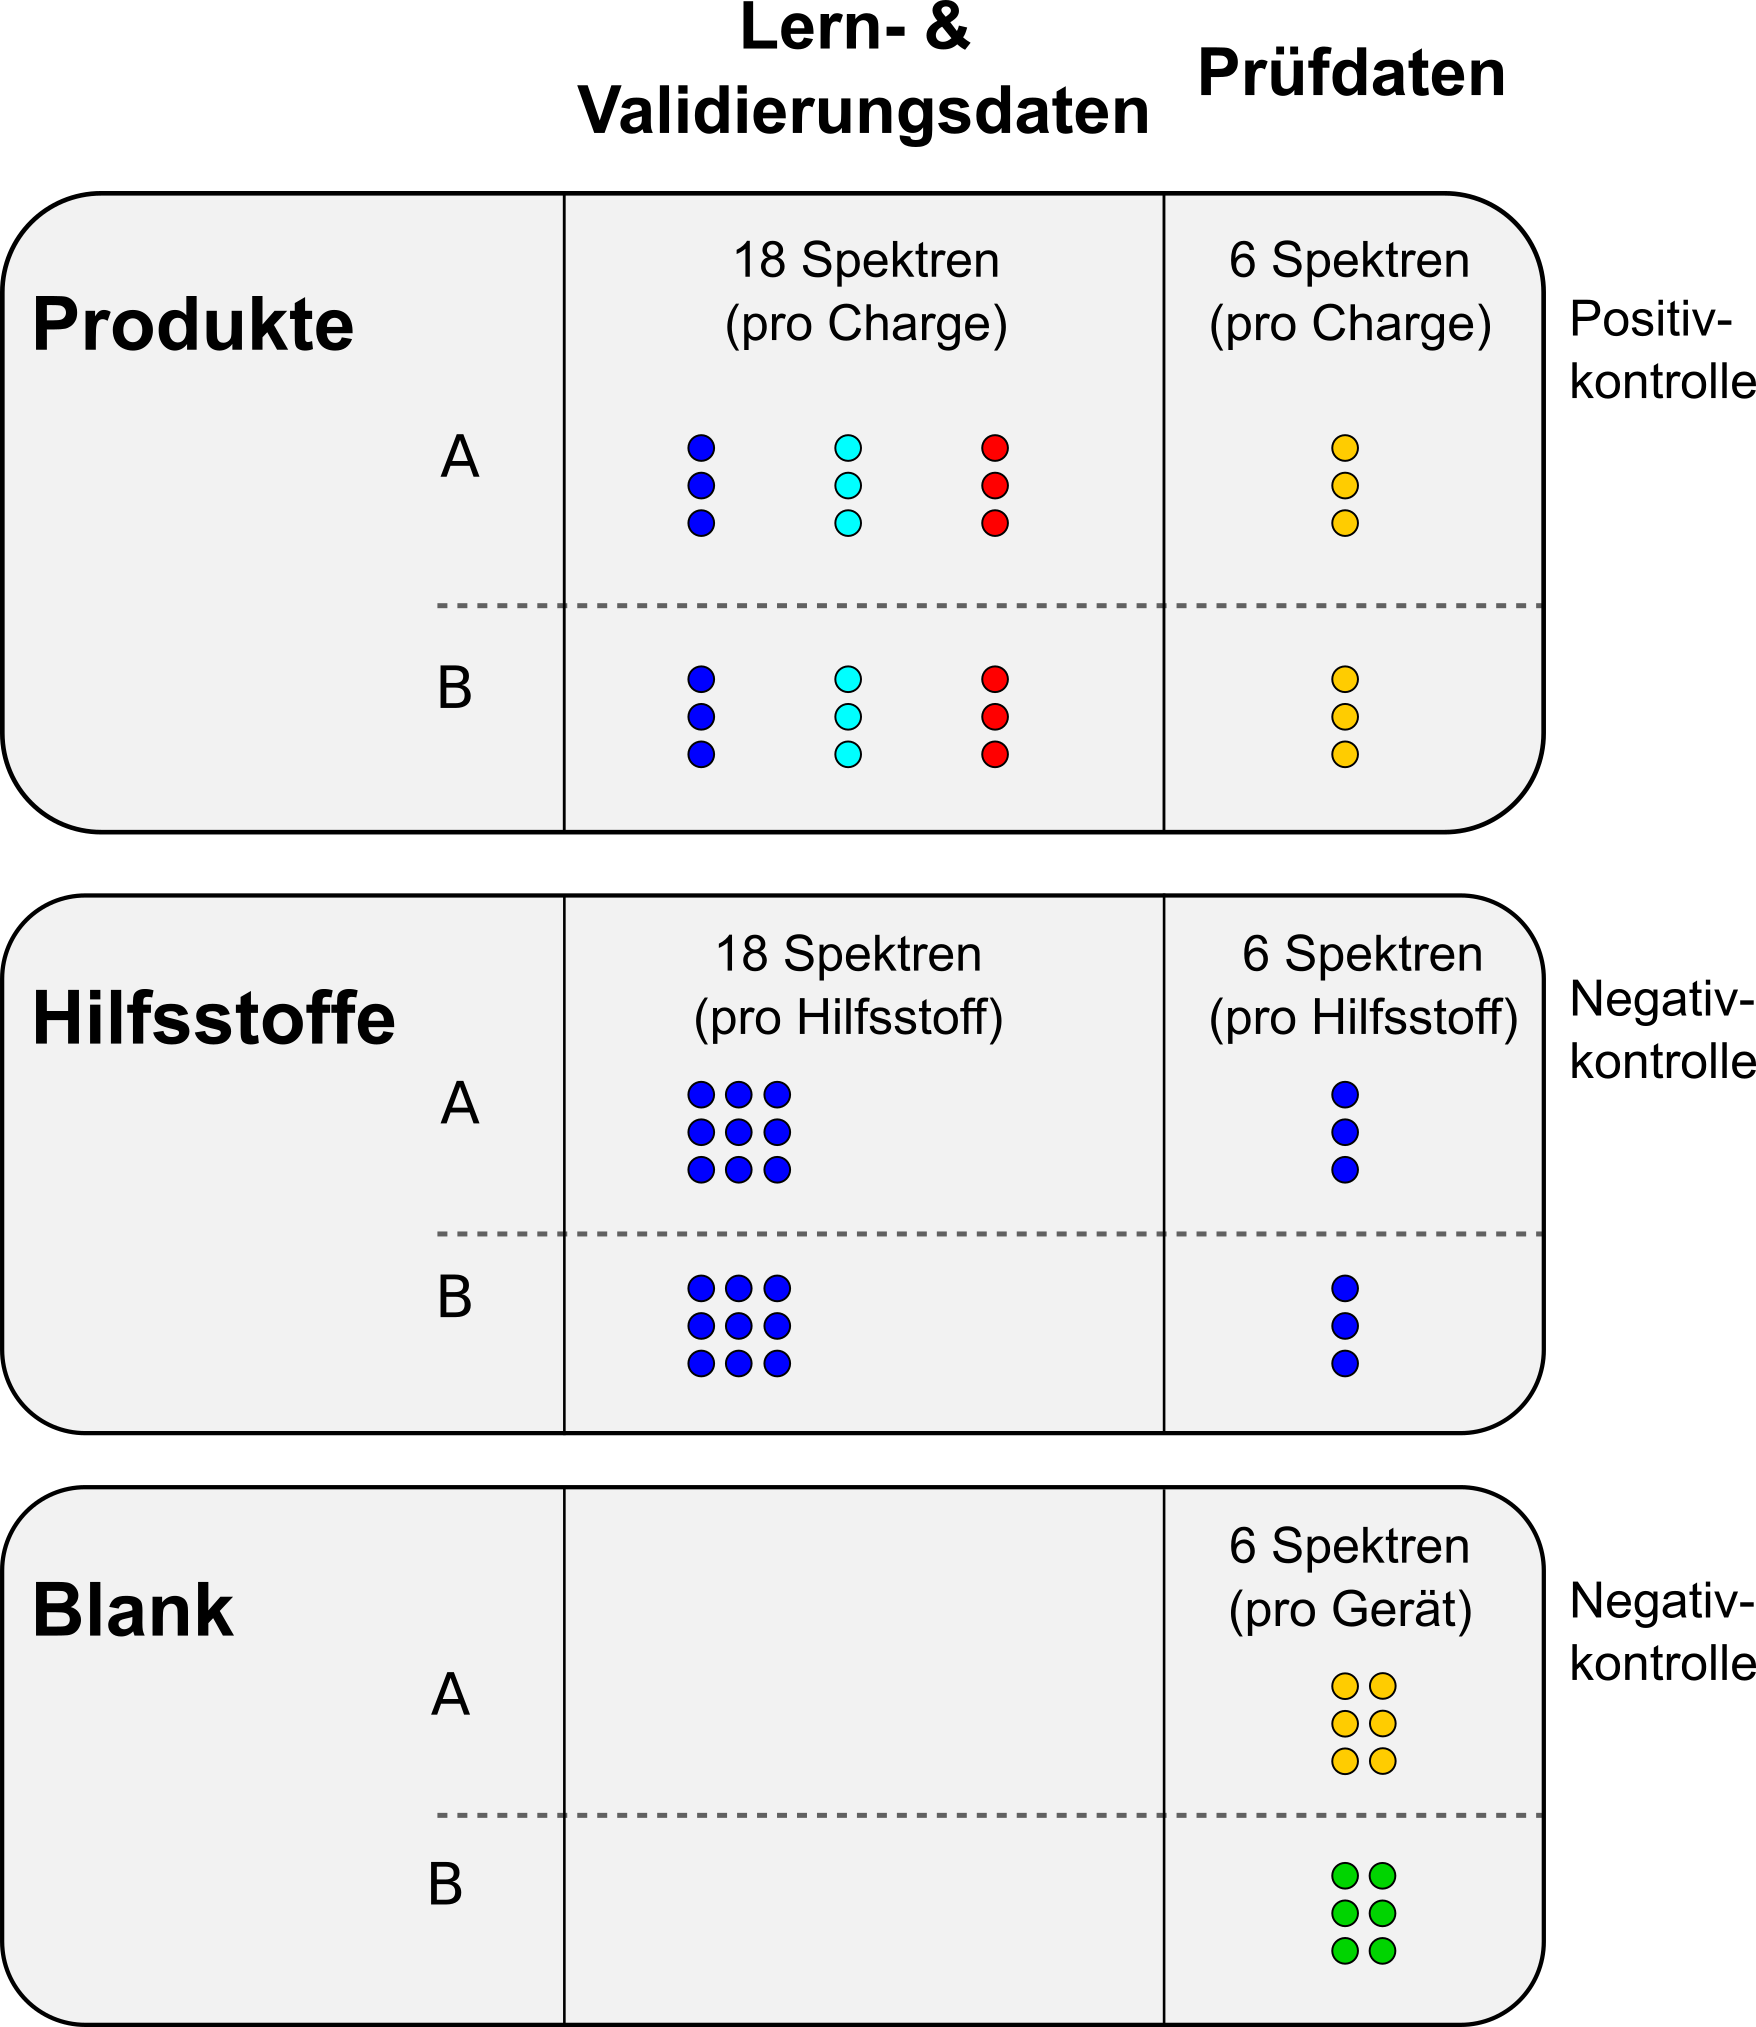
\includegraphics[width=0.8\textwidth]{sampling_design.png}
\end{center}
\caption{Übersicht zum Sampling Design. Alle Spektren werden ausgewogen auf zwei baugleichen Geräten gemessen (A/B). Die Prüfdaten der Granulatprodukte bestehen aus Messungen von Gebinden, welche nicht für die Modellierung (L/V-Daten) verwendet wurden.
Kreis = Einzelne Messung, Farbe = Unterschiedliche Gebinde, A/B = Gerätecode
}
\label{fig:Sampling_Design}
\end{figure}

\subsection{Methodenentwicklung}
PHYDENT besteht aus hierarchisch ineinander geschachtelten Künstlichen Neuronalen Netzen  (KNN). Die Methodenentwicklung erfolgte nach internem Qualitätsmanagementsystem (SOP 3.7.3) sowie den Bestimmungen des jeweils gültigen Europäischen Arzneibuchs (5.21). Anhang 1 beschreibt die einzelnen relevanten Bestimmungen des Europäischen Arzneibuchs hinsichtlich der Entwicklung chemometrischer Verfahren (5.21), und erläutert, wie diese für die vorliegende Methode berücksichtigt wurden. Anhang 2 beschreibt die einzelnen relevanten Bestimmungen des Europäischen Arzneibuchs zur Verwendung der Infrarot-Spektroskopie (2.2.24), und diskutiert wie diese für PHYDENT berücksichtigt wurden. Die Datenanalyse sowie die Entwicklung der Methode erfolgte unter Zuhilfenahme von NeuroDeveloper (Synthon Analytics, Deutschland) und R (R Core Team 2020).

\subsection{Systemeignungstest}
Die Kontrolle der Leistungsfähigkeit der Spektrometer erfolgt laufend gemäß Europäischem Arzneibuch (10.5; 2.2.24). Dazu gehören regelmäßige (wöchentliche bzw. jährliche) Performance Qualification (PQ) und Operational Qualification (OQ) Tests mit geräteinternen Testroutinen. Die Tests umfassen die Prüfpunkte 1) Richtigkeit der Wellenzahlskala (Polystyrol/Wasserdampf); 2) Spektrale Auflösung; 3) 100\%-Linie; 4) Empfindlichkeit; sowie 5) Signal-Rauschen-Verhältnis.


\section{Vorgehen}
Die Methodenvalidierung erfolgt gemäß internationalen Richtlinien (ICH Guideline Q2R1) sowie dem aktuellem Europäischem Arzneibuch (10.5). Die für die Validierung relevanten Prüfpunkte umfassen Selektivität/Spezifität und weitere kritische Parameter. Robustheit (Probentemperatur und Probenfeuchtigkeit) werden als nicht kritisch erachtet (s. Kapitel 1.8). In Anlehnung an die Bestimmungen des Europäischen Arzneibuchs (5.21) wird der gesamte Datensatz unterteilt in 1) Lerndaten, 2) Validierungsdaten und 3) Unabhängige Prüfdaten

\begin{figure}[h]
\begin{center}
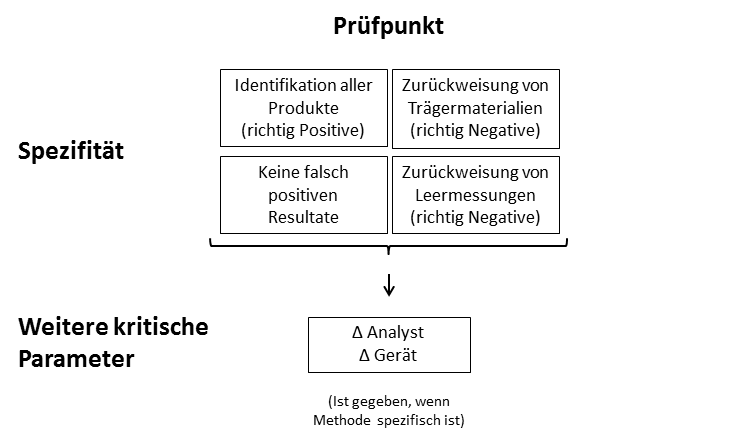
\includegraphics[width=0.8\textwidth]{flussdiagram2.png}
\end{center}
\caption{Flussdiagramm zur Überprüfung der einzelnen Parameter}
\label{fig:Sampling_Design}
\end{figure}

\subsection{Selektivität / Spezifität}
Die Validierung von Identifikationsmethoden verlangt gemäß ICH Richtlinien den Nachweis von Selektivität/Spezifität, wobei eine Methode nur dann selektiv/spezifisch ist, wenn sie die Analyten eindeutig von zu erwartenden anderen Analyten bzw. Verfälschungen unterscheidet (ICH Guideline Q2R1). Für die vorliegende Validierung wurde Selektivität der Methode folgendermaßen definiert:
\begin{enumerate}
\item 	Fähigkeit, alle unterstützten Granulatprodukte korrekt zu identifizieren;
\item 	Fähigkeit, zu erwartende Verfälschungen (Hilfsstoffe und Produkte mit künstlich beigemischtem Hilfststoff) korrekt zurückzuweisen;
\item	Fähigkeit, Leermessungen korrekt zurückzuweisen.
\end{enumerate}

\subsection{Robustheit}
\textbf{Probentemperatur}\\[1.2pt]
Probentemperatur wird als nicht kritisch erachtet, da aufgrund der geringen Probenmenge sowie der Messtechnik (ATR, abgeschwächte Totalreflexion) davon ausgegangen werden kann, dass sich die Temperatur der Probe während des Messvorgangs jener des Geräts angleicht (Anhang 8).

\textbf{Probenfeuchtigkeit}\\[1.2pt]
Probenfeuchtigkeit wird ebenfalls als nicht kritisch betrachtet, da die Versiegelung von Probengebinden gemäß Verwendungsszenario jeweils unmittelbar vor der Messung entfernt wird. Einfluss von Variation in Probenfeuchtigkeit auf das Mess- und Analyseergebnis kann somit ausgeschlossen werden (Anhang 8).


\subsection{Weitere kritische Parameter}

\subsection{Prüfkriterien}

\section{Aktzeptanzkriterien}

\subsection{Vorgehen}

\section{Dokumentation, Auswertung und Validierungsbericht}

\section{Besondere Bestimmungen}

\section{Verantwortlichkeiten}

\section{Geräte und Software}

\section{Referenzen und mitgeltende Unterlagen}

\section{Anhangsverzeichnis}


\end{document}
